\documentclass{article}
\usepackage{graphicx}
\usepackage[margin=0.75in]{geometry}
\usepackage{placeins}

\begin{document}

\title{US county-level variation in characteristics influencing participation in outdoor recreation}
\author{Abhishek Bhatia}
\date{BIOS 611 - Fall 2021}
\maketitle


\section{Background}


The term ``Nature Gap'' sheds light on the racial and economic disparities in access to greenspace, unequal distribution of nature, and the unjust experience of people of color in the outdoors across the United States. Systematic practices such as economic segregation, redlining, forced migration, racial violence, and intimidation in the outdoors have been prevalent for decades, have perpetuated the racial divide. Contemporary examples during the pandemic of Christian Cooper ``Birding While Black'' in Central Park, and Ahmaud Arbery murdered while jogging down a boulevard in Georgia show the risk and difficulty endured by people of color while in outdoor spaces.

Access to public open spaces provides communities with the opportunity to engage in physical activity and build community while incentivizing the conservation of biodiversity during the looming climate crisis. Factors typically influencing the use of these spaces include (but are not limited to) population demographics, proximity, and community recreational expenditure. For this analysis, we will use publicly available county-specific data to examine how these key factors influencing participation in outdoor recreation intersect with the proportion of the population that is people of color (i.e. not non-Hispanic white).

\section{\textbf{Data Sources}}
\subsection{Population demographics:}
\begin{itemize}
\item Population as of 2018 (Source: U.S. Census Bureau)
\item Percentage of residents living under the federal poverty level (Source: U.S. Census Bureau)
\item Percentage of population 65 years or older (Source: National Center for Health Statistics Bridged Race Population Estimates 2011)
\item Proportion of population that is not non-Hispanic White as determined by American Community Survey data (Source: U.S. Census Bureau)
\end{itemize}


\subsection{\textbf{Commercial recreation services (as a proxy for community recreation expenditure):}}
\begin{itemize}
\item Number of outdoor gear stores per million individuals at the county-level (Source: Yelp Business Dataset including location data, attributes, and categories)
\end{itemize}


\subsection{\textbf{Access to Parks (Park proximity)}}
\begin{itemize}
\item Proportion of individuals that live within a half-mile of a park boundary at the county-level (Source: CDC National Environmental Public Health Tracking Network (NEPHTN) Access to Parks Indicator (API))
\end{itemize}
\FloatBarrier

\section{\textbf{Statistical Analysis}}
\subsection{\textbf{Methods}}
For this analysis, we aggregated all measures to the county-level. We purposefully avoid weighting these factors relative to each other since there is no strong evidence to rigorously assign importance across categories. The analysis includes univariate maps to depict spatial heterogeneity across counties of the United States, as well as bivariate county-level maps to summarize relationships across categories. 

\subsection{\textbf{Univariate Results}}
\begin{figure}[!h] 
    \centering
    \includegraphics[width=11cm]{figures/univariate/fig_univariate_all.png}
    \caption{(A) Percentage of population 65 years or older, 2018 (Source: National Center for Health Statistics Bridged Race Population Estimates 2018, Vintage 2018). (B) Percentage of households living in poverty, 2016 (Source: CDC Atlas via the Census Small Area Income and Policy Estimates). (C) Percentage of population non-Hispanic and non-white, 2018 (Source: National Center for Health Statistics). (D) Population as of 2018 (Source: U.S. Census Bureau) (E) Proportion of individuals that live within a half-mile of a park boundary at the county-level (Source: CDC National Environmental Public Health Tracking Network (NEPHTN) Access to Parks Indicator (API). (F) Number of outdoor gear stores per million individuals at the county-level (Source: Yelp Business Dataset including location data, attributes, and categories))}
    \
\end{figure}
\FloatBarrier


\subsection{\textbf{Bivariate Results- Access to Parks}}
\begin{figure}[!h] 
    \centering
    \includegraphics[width=15cm]{figures/bivariate/fig_bivariate_api.png}
    \caption{Access to Parks indicator score (Source: CDC National Environmental Public Health Tracking Network (NEPHTN)) and: (A) Percentage of population 65 years or older, 2018 (Source: National Center for Health Statistics Bridged Race Population Estimates 2018, Vintage 2018). (B) Percentage of households living in poverty, 2016 (Source: CDC Atlas via the Census Small Area Income and Policy Estimates). (C) Percentage of population non-Hispanic and non-white, 2018 (Source: National Center for Health Statistics)}
    \
\end{figure}
\FloatBarrier

\subsection{\textbf{Bivariate Results- Access to retail}}
\begin{figure}[!h] 
    \centering
    \includegraphics[width=15cm]{figures/bivariate/fig_bivariate_retail.png}
    \caption{Number of outdoor gear stores per million individuals at the county-level (Source: Yelp Business Dataset including location data, attributes, and categories)and: (A) Percentage of population 65 years or older, 2018 (Source: National Center for Health Statistics Bridged Race Population Estimates 2018, Vintage 2018). (B) Percentage of households living in poverty, 2016 (Source: CDC Atlas via the Census Small Area Income and Policy Estimates). (C) Percentage of population non-Hispanic and non-white, 2018 (Source: National Center for Health Statistics).}
    \
\end{figure}
\FloatBarrier

\section{Supplemental Figures}
\subsection{\textbf{Univariate Figures}}
\begin{figure}[!h] 
    \centering
    \caption{Percentage of population 65 years or older, 2018 (Source: National Center for Health Statistics Bridged Race Population Estimates 2018, Vintage 2018).}
    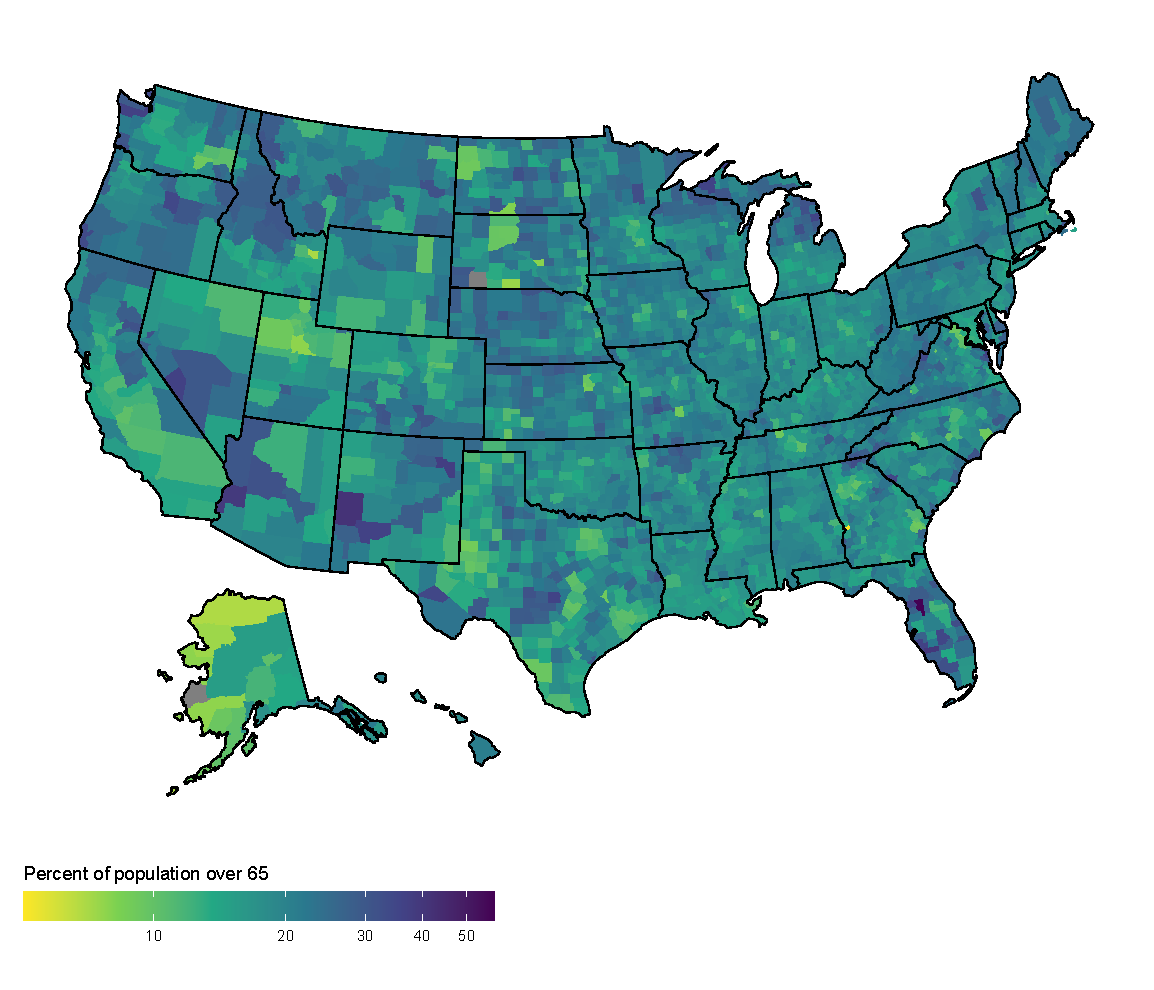
\includegraphics[width=11cm]{figures/univariate/figU01_p_65yo.png}
    \
\end{figure}
\FloatBarrier

\begin{figure}[!h] 
    \centering
    \caption{Percentage of households living in poverty, 2016 (Source: CDC Atlas via the Census Small Area Income and Policy Estimates).}
    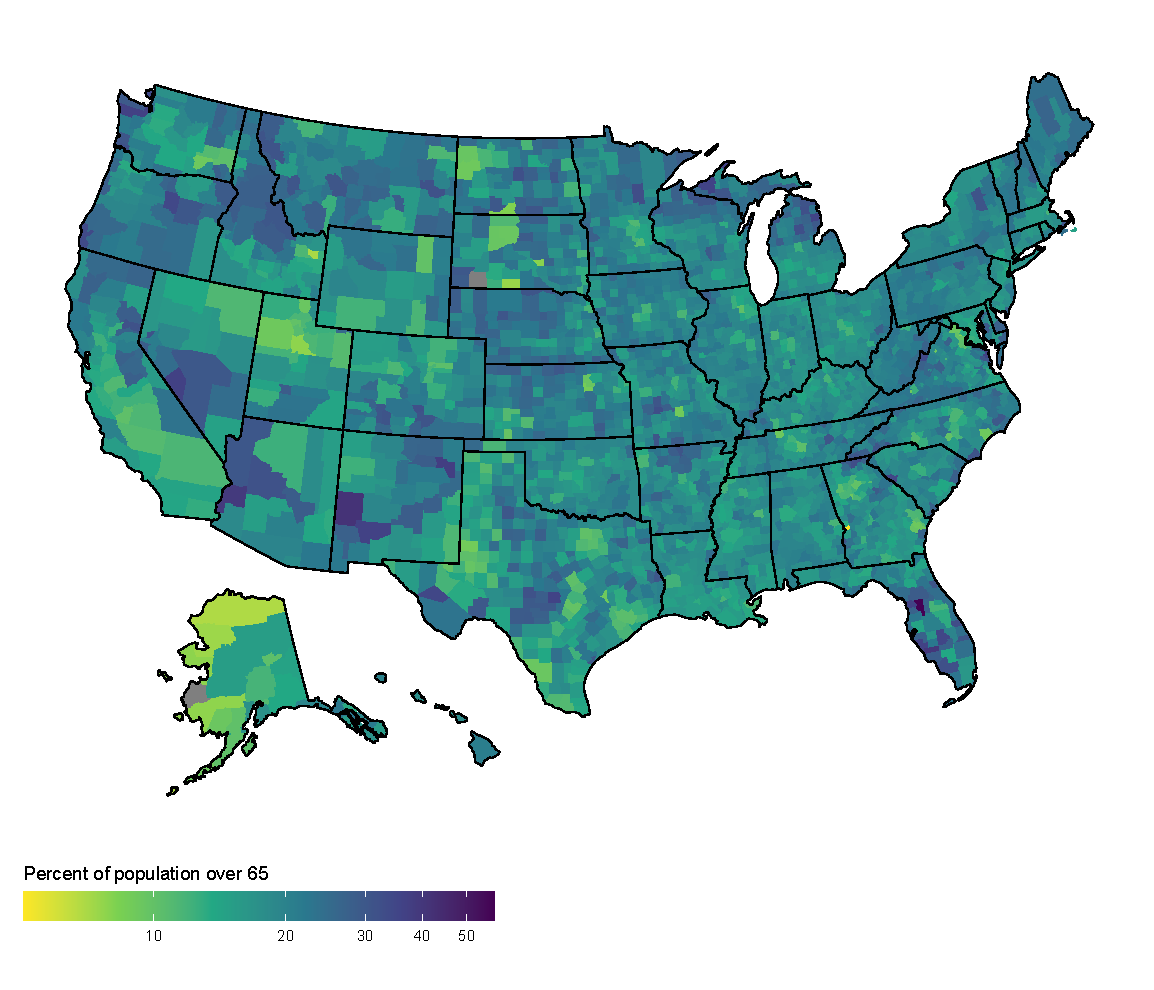
\includegraphics[width=11cm]{figures/univariate/figU02_poverty.png}
    \
\end{figure}
\FloatBarrier

\begin{figure}[!h] 
    \centering
    \caption{Percentage of population non-Hispanic and non-white, 2018 (Source: National Center for Health Statistics).}
    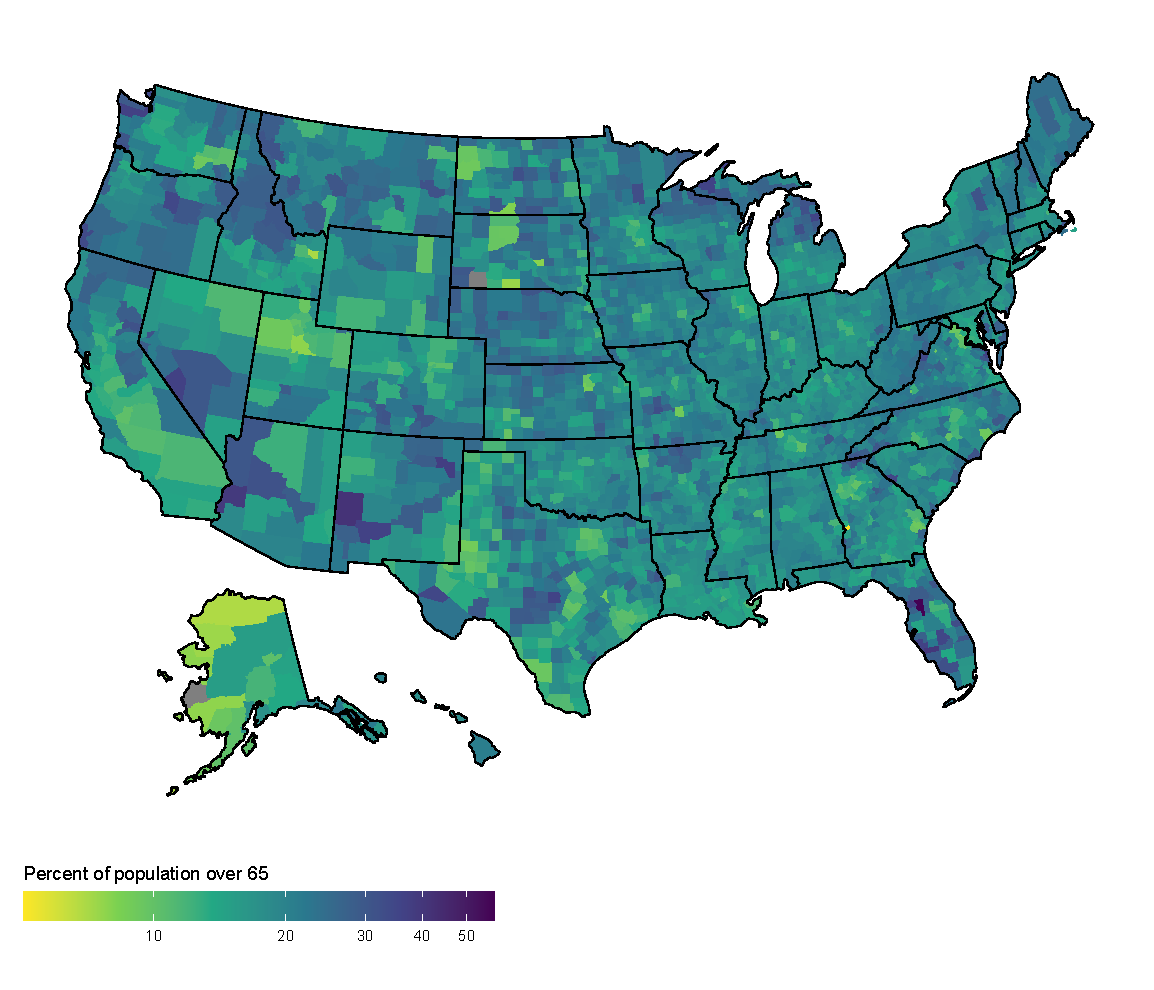
\includegraphics[width=11cm]{figures/univariate/figU03_p_nonwhite_nonhispanic.png}
    \
\end{figure}
\FloatBarrier

\begin{figure}[!h] 
    \centering
    \caption{Population as of 2018 (Source: U.S. Census Bureau)}
    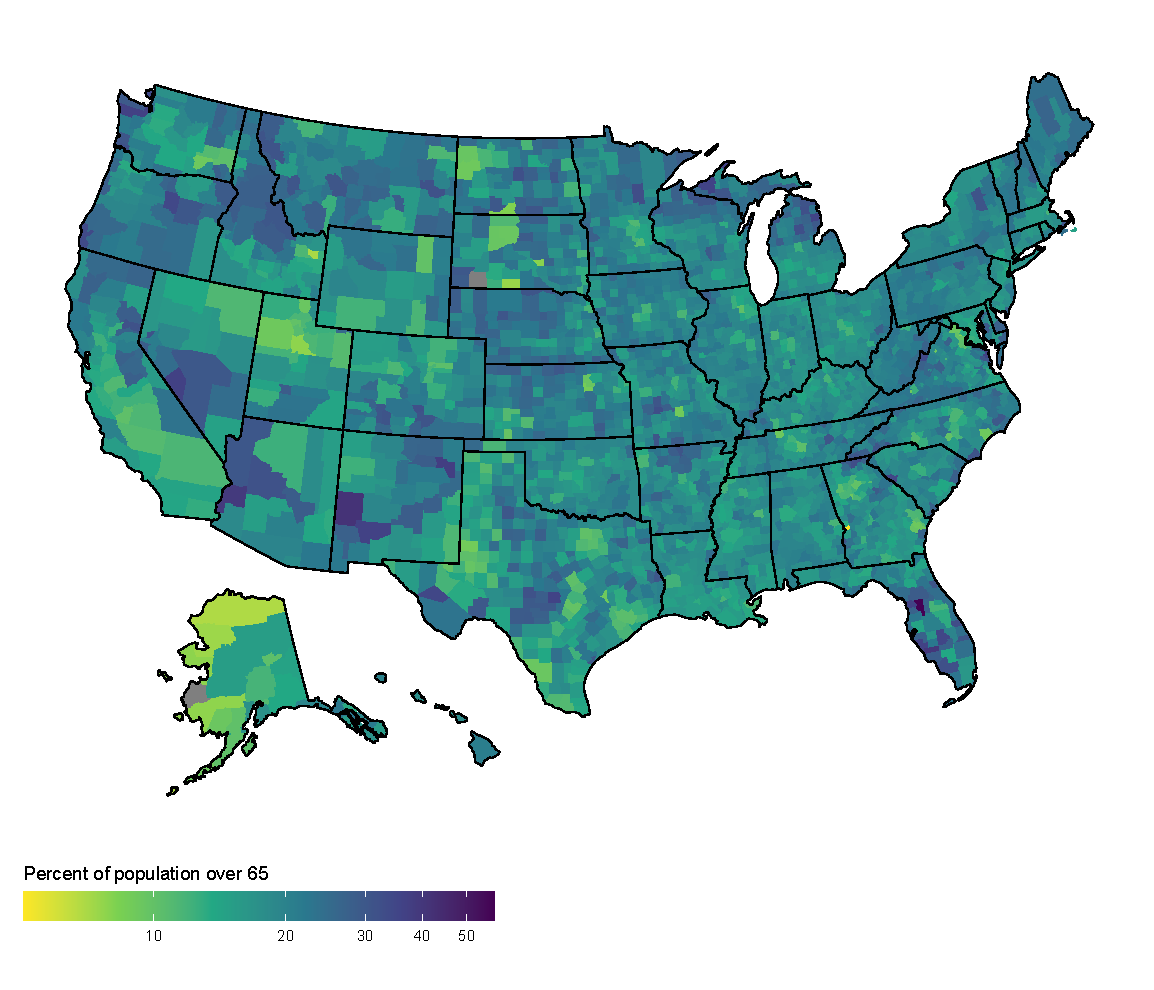
\includegraphics[width=11cm]{figures/univariate/figU04_population.png}
    \
\end{figure}
\FloatBarrier

\begin{figure}[!h] 
    \centering
    \caption{Proportion of individuals that live within a half-mile of a park boundary at the county-level (Source: CDC National Environmental Public Health Tracking Network (NEPHTN) Access to Parks Indicator (API)).}
    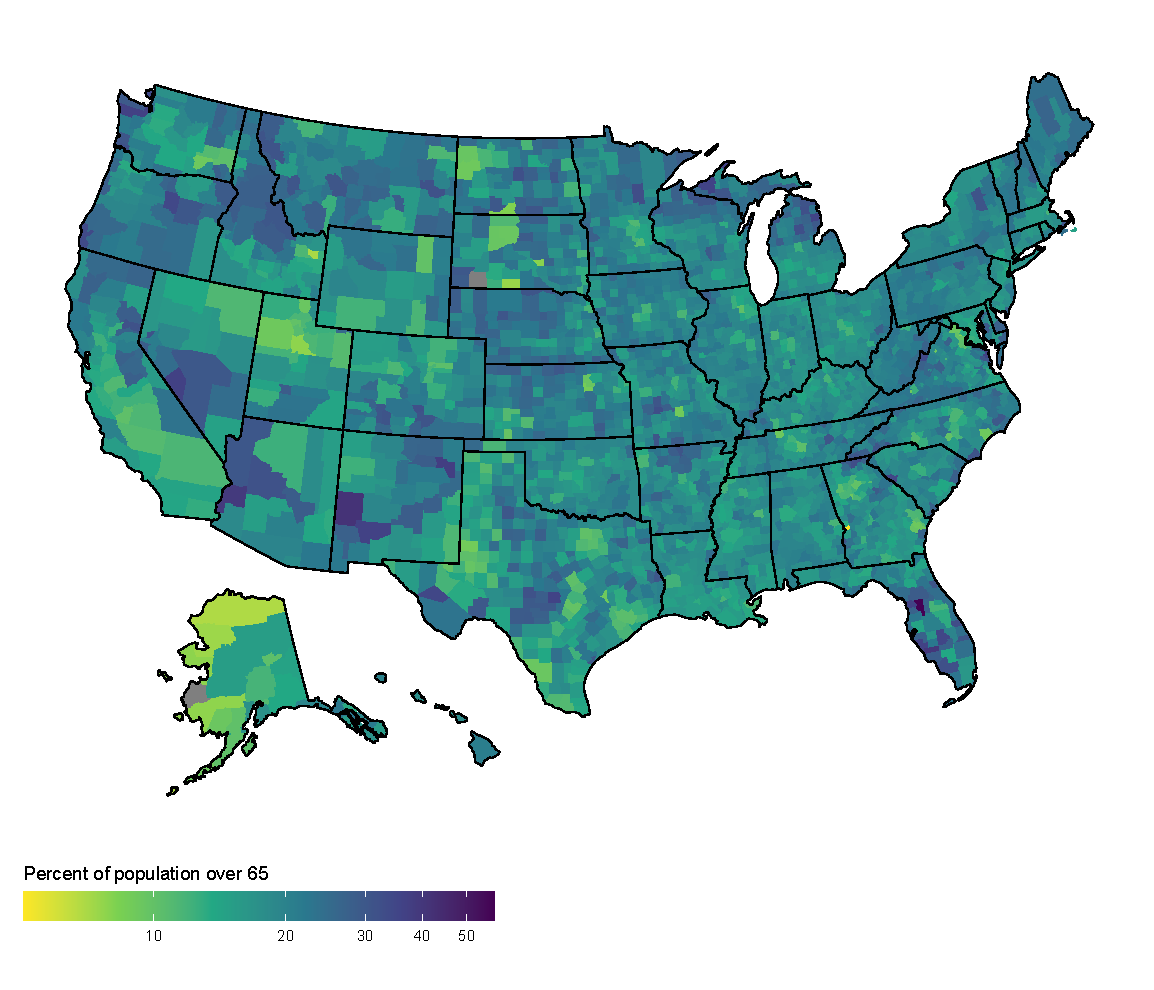
\includegraphics[width=11cm]{figures/univariate/figU05_api.png}
    \
\end{figure}
\FloatBarrier

\begin{figure}[!h] 
    \centering
    \caption{Number of outdoor gear stores per million individuals at the county-level (Source: Yelp Business Dataset including location data, attributes, and categories).}
    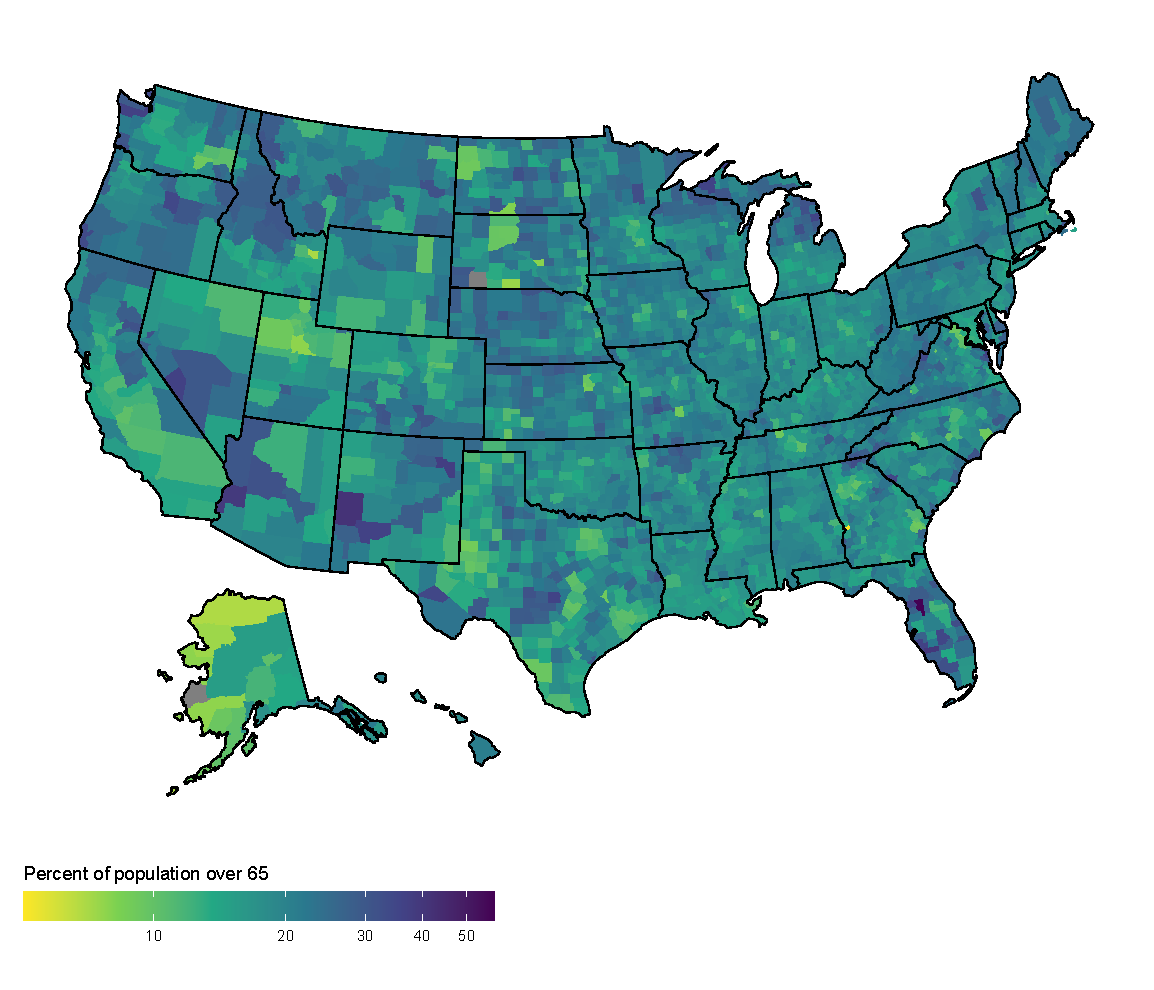
\includegraphics[width=11cm]{figures/univariate/figU06_n_businesses_permil.png}
    \
\end{figure}
\FloatBarrier

\newpage
\subsection{\textbf{Bivariate Figures}}
\begin{figure}[!h] 
    \centering
    \caption{Number of outdoor gear stores per million individuals at the county-level (Source: Yelp Business Dataset including location data, attributes, and categories) and Percentage of population 65 years or older, 2018 (Source: National Center for Health Statistics Bridged Race Population Estimates 2018, Vintage 2018). }
    \includegraphics[width=16cm]{figures/bivariate/figB01.png}
    \
\end{figure}
\FloatBarrier

\begin{figure}[!h] 
    \centering
    \caption{Number of outdoor gear stores per million individuals at the county-level (Source: Yelp Business Dataset including location data, attributes, and categories) and Percentage of households living in poverty, 2016 (Source: CDC Atlas via the Census Small Area Income and Policy Estimates).}
    \includegraphics[width=16cm]{figures/bivariate/figB02.png}
    \
\end{figure}
\FloatBarrier

\begin{figure}[!h] 
    \centering
    \caption{Number of outdoor gear stores per million individuals at the county-level (Source: Yelp Business Dataset including location data, attributes, and categories) and Percentage of population non-Hispanic and non-white, 2018 (Source: National Center for Health Statistics).}
    \includegraphics[width=16cm]{figures/bivariate/figB03.png}
    \
\end{figure}
\FloatBarrier

\begin{figure}[!h] 
    \centering
    \caption{Proportion of individuals that live within a half-mile of a park boundary at the county-level (Source: CDC National Environmental Public Health Tracking Network (NEPHTN) Access to Parks Indicator (API)) and Percentage of population 65 years or older, 2018 (Source: National Center for Health Statistics Bridged Race Population Estimates 2018, Vintage 2018). }
    \includegraphics[width=16cm]{figures/bivariate/figB04.png}
    \
\end{figure}
\FloatBarrier

\begin{figure}[!h] 
    \centering
    \caption{Proportion of individuals that live within a half-mile of a park boundary at the county-level (Source: CDC National Environmental Public Health Tracking Network (NEPHTN) Access to Parks Indicator (API)) and Percentage of households living in poverty, 2016 (Source: CDC Atlas via the Census Small Area Income and Policy Estimates).}
    \includegraphics[width=16cm]{figures/bivariate/figB05.png}
    \
\end{figure}
\FloatBarrier

\begin{figure}[!h] 
    \centering
    \caption{Proportion of individuals that live within a half-mile of a park boundary at the county-level (Source: CDC National Environmental Public Health Tracking Network (NEPHTN) Access to Parks Indicator (API)) and Percentage of population non-Hispanic and non-white, 2018 (Source: National Center for Health Statistics).}
    \includegraphics[width=16cm]{figures/bivariate/figB06.png}
    \
\end{figure}
\FloatBarrier


\end{document}
